% !TeX root = main.tex


\begin{savequote}[70mm]
,,Jeżeli zabałaganione biurko jest znakiem zabałaganionego umysłu, znakiem czego
jest puste biurko?''
\qauthor{Albert Einstein}
\end{savequote}


\chapter{Opis systemu sterowania}
\label{chap:software}

\section{Dekompozycja zadania}

Całe zadanie sterowania robota zostało rozdzielone na moduły odpowiedzialne
za poszczególne fragmenty systemu -- lokalizację robota (lokalną i globalną), 
wykrywanie przeszkód (przez oba dostępne sensory -- skaner laserowy i Kinect),
sterowanie samym robotem (poruszanie bazy jezdnej) oraz diagnostykę.

\begin{figure}[ht!]
\centering
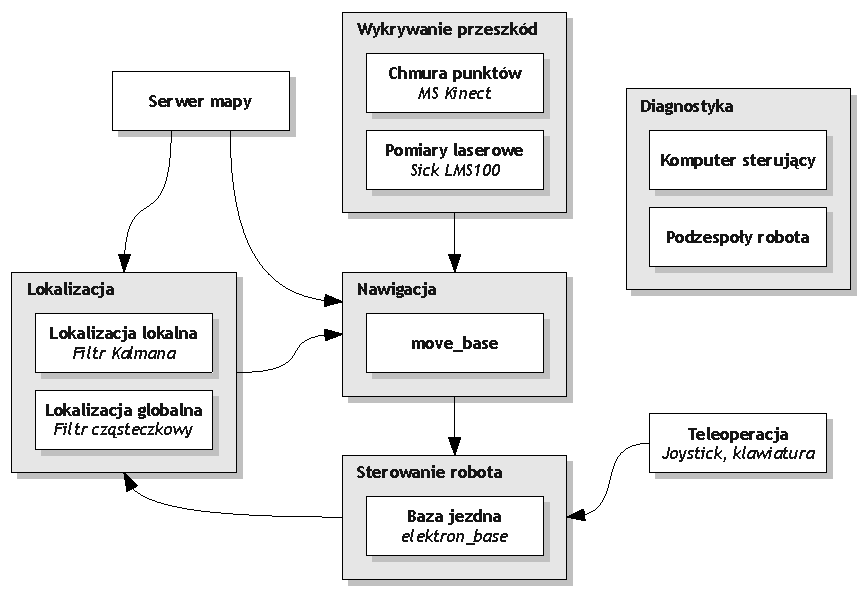
\includegraphics{../img/decomposition}
\caption{Dekompozycja systemu sterowania robota}
\label{fig:decomposition}
\end{figure}

Rysunek~\ref{fig:decomposition} przedstawia najważniejsze moduły systemu,
wraz z ogólnymi zależnościami pomiędzy nimi. Najważniejsze podsystemy
są opisane w dalszej części pracy. 

Taki podział systemu pozwala na zmniejszenie zależności pomiędzy jego elementami
do niezbędnego minimum. Poszczególne moduły komunikują się ze sobą przy pomocy 
ogólnie określonych interfejsów, a format konkretnych komunikatów nie jest 
zależny od modelu sprzętu, który jest używany do ich wygenerowania. Dzięki temu
zmiana dowolnego elementu nie wymaga wprowadzania zmian w pozostałych,
podobnie dodawanie nowych modułów (np. sensorycznych). Jest to podstawowe
wymaganie przy tworzeniu platform badawczych, na których można testować różne
algorytmy, m.in. sterowania ruchem robota, lokalizacji czy przetwarzania danych
w celu wykrywania przeszkód. 


\section{Obliczanie położenia robota}

Kluczowym zadaniem podczas pracy robota mobilnego jest określenie jego
aktualnego położenia, w układzie współrzędnych bądź to bezwzględnym (o początku
w pewnym ustalonym punkcie, np. położenie w budynku czy globalna pozycja
geograficzna) bądź pozycji względem punktu, z którego robot wystartował.
Możliwości pozycjonowania bezwzględnego wewnątrz budynków są ograniczone w
stosunku do przestrzeni otwartych. W budynkach nie sprawdza się GPS, utrudnione
jest nawigowanie względem nadajników GSM (dodatkowo jego dokładność jest dużo
za mała). Lokalizacja na podstawie naturalnych cech otoczenia w budynkach o
charakterze biurowym często może być błędna ze względu na istnienie wielu miejsc
o cechcach podobnych bądź wyglądających wręcz identycznie (np. korytarze na
różnych piętrach). Istnieją metody lokalizacji na podstawie sztucznie
umieszczonych znaczników, jednak zgodnie z założeniami zadania robot ma poruszać
się w środowku, które nie jest specjalnie przygotowane (a więc metody oparte o
pozycjonowanie względem latarni podczerwonych czy innych znaczników odpadają).
Z tego względu globalna pozycja robota nie jest wyznaczana, a podczas
autonomicznego dojazdu do celu rolą użytkownika jest wskazanie na mapie
przybliżonego punktu, z którego robot startuje.

W przypadku jeżdżących robotów mobilnych operujących w przestrzeniach
zamkniętych najczęściej wystarcza określenie dwuwymiarowego położenia i
orientacji robota, określonego trójką liczb $(x, y, \theta)$. W przypadku
robota Elektron dostępne są trzy niezależne źródła informacji o jego położeniu
względnym (dwa zwracające pełną trójkę, jedno określające jedynie bieżącą
orientację). Dokonując fuzji informacji uzyskiwanych ze wszystkich źródeł można
radykalnie zwiększyć jej dokładność. Rysunek~\ref{fig:diag_pos} przedstawia
przepływ danych pomiędzy modułami odpowiedzialnymi za kolejne etapy lokalizacji
robota, a każdy z nich jest opisany dokładniej w dalszej części rozdziału.

\begin{figure}[h!]
\centering
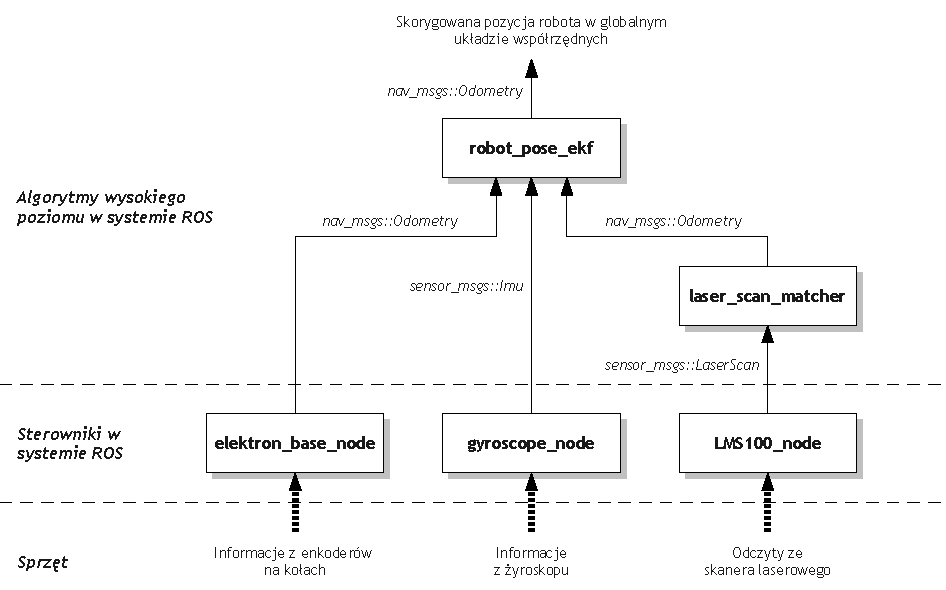
\includegraphics{../img/diag_position}
\caption{Hierarchia zadań obliczania bieżącej pozycji robota}
\label{fig:diag_pos}
\end{figure}

\subsection{Odometria}

Pierwszym źródłem informacji o położeniu robota jest moduł napędowy robota.
Wyposażony jest on w enkodery mierzące aktualną pozycję kół, dzięki czemu na
bieżąco obliczać można dystans, jaki pokonał robot. Istnieją proste wzory, które
przy znajomości chwilowej zmiany położenia kół lewej i prawej strony robota
pozwalają określić zmianę położenia i orientacji robota. Sterownik silników
robota Elektron zwraca właśnie taką informację (dokładniej ilość impulsów
enkodera zliczoną dla każdego z kół za jeden okres regulacji), oznaczmy ją przez
$(\Delta N_L, \Delta N_R)$.

\subsubsection{Obliczenie przyrostu pozycji}

Załóżmy, że w okresie $I$ sterownik silników zliczył i zwrócił do systemu
sterowania liczbę impulsów dla lewego i prawego koła $(\Delta N_L, \Delta N_R)$.
Znając dodatwe parametry:

% TODO: ładniejsze wyrównanie spisu symboli

\begin{mydescription}{5pt}
\item[$N$] liczba impulsów enkodera na pełny obrót koła,
\item[$d$] średnica koła,
\item[$b$] odstęp pomiędzy kołami robota, 
\end{mydescription}

można obliczyć dystans, jaki przebyły koła po każdej ze stron robota:

\[
\Delta S_{L,R} = \frac{\pi D}{N} \cdot \Delta N_{L,R}
\]

skąd łatwo można policzyć przesunięcie środka robota oraz zmianę jego
orientacji:

\begin{align*}
\Delta S_i &= \frac{\Delta S_L + \Delta S_R}{2} \\
\Delta \theta_i &= \frac{\Delta S_L - \Delta S_R}{b}
\end{align*}

Przy odpowiednio krótkim okresie próbkowania danych z enkoderów można założyć,
że droga pokonana przez robota w tym czasie jest odcinkiem prostej, co pozwala w
łatwy sposób obliczyć zmianę pozycji i orientacji robota:

\begin{align*}
\theta_i &= \theta_{i-1} + \Delta \theta_i \\
x_i &= x_{i-1} + \Delta S_i \cdot cos(\theta_i) \\ 
y_i &= y_{i-1} + \Delta S_i \cdot sin(\theta_i) 
\end{align*}


\subsubsection{Źródła błędów}

Odometria opiera się na bardzo prostych równaniach, dodatkowo polegając na
uproszczeniu zakładającym, że obrót koła przekłada się dokładnie na pokonany
przez nie dystans. Założenie to często się nie sprawdza, wymienić można
chociazby przypadek poślizgu kół. Wszystkie źródła błędów można zgrupować w
dwóch kategoriach: błędy systematyczne i niesystematyczne~\cite{whereami}.
Błędy z pierwszej grupy kumulują się w przybliżeniu jednostajnie przez cały czas
działania robota, przez co mogą zostać zniwelowane przez odpowiednie kalibracje.
Do błędów tych zalicza się:
\begin{itemize}
  \item faktyczna średnica kół inna od założonej,
  \item różna średnica kół po lewej i prawej stronie robota,
  \item faktyczny odstęp pomiędzy kołami różny od założonego,
  \item osie obrotu kół nie są współliniowe,
  \item skończona rozdzielczość enkoderów,
  \item częstotliwość próbkowania enkoderów.
\end{itemize}

Błędy niesystematyczne z kolei są w swej naturze nieprzewidywalne, a ich
zniwelowanie podczas działania robota jest praktycznie niemożliwe. Źródłami
błędów z tej kategorii są:
\begin{itemize}
  \item nierówności podłoża,
  \item najechanie na przeszkody,
  \item poślizgi wywołane:
  \begin{itemize}
    \item niską przyczepnością kół do podłoża,
    \item dużym przyspieszeniem,
    \item szybkimi skrętami,
    \item działaniem sił zewnętrznych,
    \item nie-punktowym kontaktem kół z podłożem.
  \end{itemize}
\end{itemize}

Występowanie tego typu błędów jest w dużym stopniu zależne od środowiska, w
jakim porusza się robot. W przypadku robota Elektron, jego sześciokołowa
konstrukcja sprzyja występowaniu problemów z tej grupy. Środek obrotu przesuwa
się w zależności od chwilowego kontaktu kół z podłożem, przez co w trakcie
obracania się może się zdarzyć, że robot oprócz orientacji zmienia także
położenie (co nie jest wykryte przez odometrię).

\subsubsection{Kalibracja}

Kilka z wymienionych wcześniej błędów można starać się zniwelować używając
stosunkowo prostych metod. Kalibracja dokładnej wielkości kół polega na
przejechaniu odcinka prostego o znanej długości, a następnie odczytaniu tej
wielkości z odometrii. Stosunek tych danych stanowi współczynnik skalujący
składowej liniowej. Współczynnik składowej kątowej (a więc kalibrację długości
osi) oblicza się wykonując robotem obrót o znany kąt (np. dwa pełne obroty,
czyli 720\textdegree), a następnie dzieląc tę wielkość przez wartość obrotu
odczytaną z odometrii. Procedura ta została wykonana dla robota Elektron, a jej
rezultaty pokazane są na wykresie~\ref{fig:odom_calib}.

\begin{figure}[ht!]
\centering
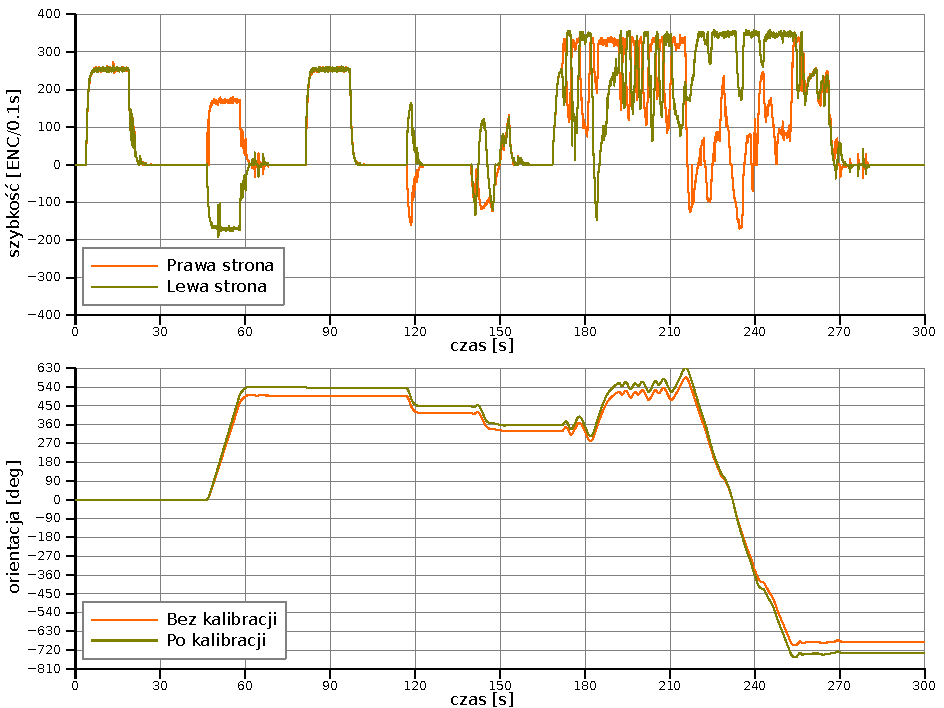
\includegraphics[width=\textwidth]{../../Common/pomiary/odom_calib}
\caption{Kalibracja odometrii robota}
\label{fig:odom_calib}
\end{figure}

\subsection{Pomiary z żyroskopu}

Korzystając z modułu wyposażonego w żyroskop można mierzyć prędkość kątową
$\omega$ robota, a z niej można sukcesywnie wyznaczać jego orientację. Wzory w
tym przypadku również nie są złożone i sprowadzają się do przemnożenia chwilowej
wartości prędkości przez czas, jaki upłynął od ostatniego pomiaru. 

\subsubsection{Źródła błędów}

Podstawowymi źródłami błędów pojawiających się podczas pomiarów przy użyciu
żyroskopów piezoelektrycznych są:

\begin{itemize}
  \item przesunięcie poziomu zera,
  \item niedokładnie dobrany współczynnik skalowania,
  \item dryf związany z temperaturą układu,
  \item dryf wartości w czasie,
  \item wpływ przyspieszenia na podawaną wartość.
\end{itemize}

Dodatkowe błędy są wnoszone przez układ konwertera analogowo-cyfrowego
(zastosowany na robocie żyroskop zwraca pomiary w postaci napięciowej).
Wiele z wymienionych błędów można zminimalizować wykonując odpowiednią
kalibrację układu pomiarowego.

\subsubsection{Kalibracja}

Wykorzystany w projekcie żyroskop ma liniową charakterystykę zależności
wartości napięcia na wyjściu od prędkości kątowej. Można ją zapisać w postaci:

\[
\omega = a \cdot (U - b)
\]

gdzie:

\begin{mydescription}{5pt}
\item[$\omega$] prędkość kątowa żyroskopu,
\item[$U$] wartość napięcia zwracana przez żyroskop,
\item[$a$] współczynnik skalujący 
\item[$b$] składowa stała pomiaru. 
\end{mydescription}

\begin{figure}[htp!]
\centering
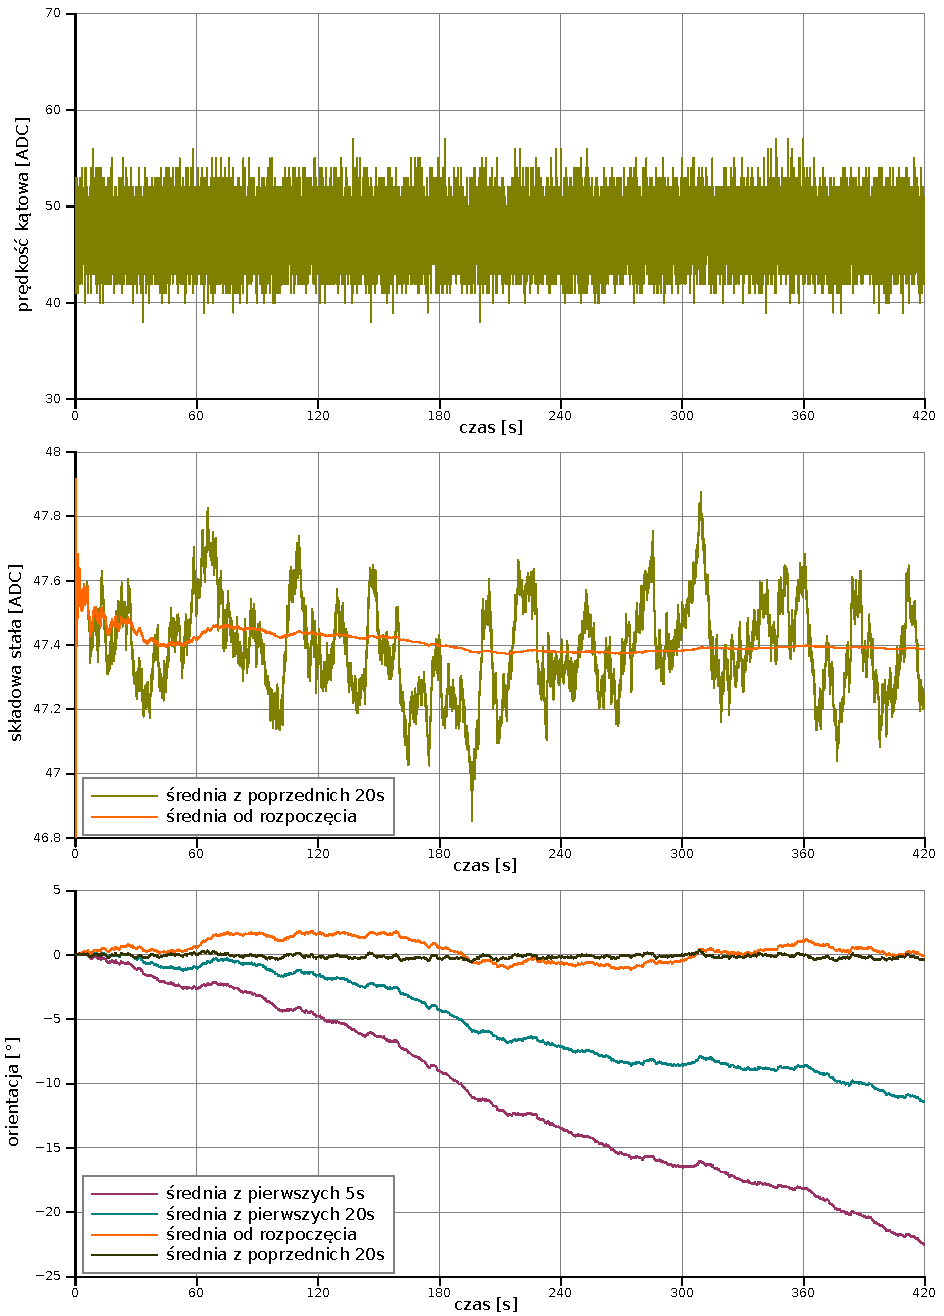
\includegraphics[width=15.5cm]{../../Common/pomiary/gyro_bias}
\caption{Kalibracja składowej stałej żyroskopu}
\label{fig:gyro_bias}
\end{figure}

Wyznaczenie składowej stałej nie jest (wbrew pozorom) zadaniem prostym. Układy
żyroskopów zrealizowane w technologii MEMS (a taki jest zastosowany)
charakteryzują się pływającą wartością składowej stałej. Prostym sposobem jej
estymacji jest uśrednienie kilkuset pierwszych pomiarów w czasie, kiedy
robot jest nieruchomy (jego prędkość kątowa jest zerowa), a następnie
traktowanie tej wartości jako składowej stałej w dalszej pracy. Niestety --
takie rozwiązanie sprawdza się jedynie na krótką metę, a w czasie pracy
orientacja robota obliczana z wykorzystaniem tego parametru zacznie coraz
bardziej oddalać się od wartości rzeczywistej. Na rysunku~\ref{fig:gyro_bias}
przedstawione są pomiary zebrane z żyroskopu przez 6 minut pracy, kiedy robot
był całkowicie nieruchomy (górny wykres, wartością oczekiwaną jest prędkość
zerowa). Środkowy wykres przedstawia średnią wartość tych pomiarów (a więc
składową stałą kumulowaną dla kolejnych pomiarów). Widać wyraźnie, że wartość ta
nie jest stabilna i podlega fluktuacjom o niekreślonej charakterystyce. Ostatni
wykres przedstawia wartość orientacji robota liczoną dla kilku długości czasu
interpolacji składowej stałej przed pomiarami (5, 20 i 120 sekund) oraz dla
składowej stałej liczonej ze wszystkich dostępnych próbek (takie rozwiązanie
nie jest możliwe do zastosowania przy pracy on-line). 

Z przedstawionego wykresu wynika, że pomiar składowej stałej jest prawidłowy dla
krótkich okresów tuż po jego wykonaniu, a wraz z upływem czasu oorientacja
robota coraz bardziej oddala się od wartości prawidłowej. Prostym sposobem na
zwalczenie tego efektu może być wykorzystanie dodatkowej informacji o braku
ruchu robota (np. z odometrii) i przeliczanie współczynnika składowej stałej
właśnie w tych momentach.

\begin{figure}[ht!]
\centering
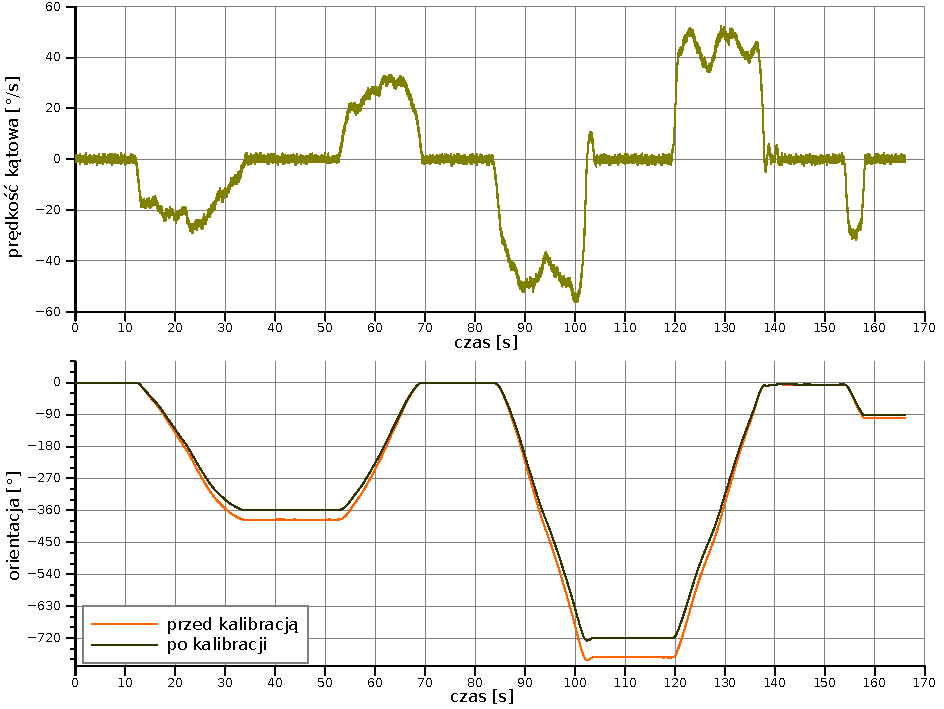
\includegraphics[width=\textwidth]{../../Common/pomiary/gyro_rot}
\caption{Kalibracja współczynnika skalowania żyroskopu}
\label{fig:gyro_rot}
\end{figure}

Drugim współczynnikiem związanym z przeliczaniem wartości napięcia zwracanego
przez żyroskop na prędkość kątową jest współczynnik skalowania. Tutaj kalibracja
jest prostsza, gdyż wartość tego parametru jest w przybliżeniu stała w czasie
dla danego układu (zależy od temperatury, ale zgodnie z założeniami robot
porusza się w obrębie pomieszczeń zamkniętych, gdzie różnice temperatur sa
niewielkie). Możliwe są dwie relatywnie proste metody kalibracji: pierwsza z
nich polega na umieszczeniu układu z żyroskopem na stoliku obrotowym i obracanie
nim ze stałą, znaną prędkością. Współczynnik skalowania wylicza się dzieląc
prędkość zadaną przez prędkość odczytaną z układu. Wadą tego rozwiązania jest po
pierwsze konieczność posiadania stolika obrotowego, po drugie problem z
ułożeniem przewodów podczas obrotów (ew. konieczność obrotu całego, ciężkiego
robota). Drugą metodą, dającą tak samo dobre rezultaty, jest obrócenie robota o
znany kąt, a następnie obliczenie szukanego parametru jako stosunku tego kąta do
skumulowanej wartości obrotu odczytanej z żyroskopu. Właśnie takie rozwiązanie
zostało zastosowane w projekcie.

Wykres~\ref{fig:gyro_rot} przedstawia odczyty z procesu kalibracji (do
policzenia współczynnika składowej stałej wybrany został okres pierwszych 10
sekund). Pierwszy wykres przedstawia wartość prędkości kątowej odczytanej z
żyroskopu (stosując domyślny współczynnik skalowania dla tego układu wynoszący
$15mV/{}^o/s$). Podczas kalibracji robot został obrócony o pełny obrót w
lewo, następnie pełny obrót w prawo, później kolejno dwa razy w lewo, dwukrotnie
w prawo, i na końcu o 90\textdegree w lewo. Oczekiwane wartości orientacji w tym
procesie wynosiły kolejno -360\textdegree, 0\textdegree, -720\textdegree,
0\textdegree, -90\textdegree. Wartości odczytane w punktach charakterystycznych
wynosiły: -385.743\textdegree, 0.047\textdegree, -774.087\textdegree,
-5.743\textdegree, -98.677\textdegree. Wartość współczynnika skalującego została
wyliczona z trzeciego odczytu:

\[
a = \frac{720^o}{774.087^o} = 0.930
\]

Orientacja robota z uwzględnionym współczynnikiem skalującym zostala
przedsationa na wspólnym wykresie razem z wartościami pierwotnymi. Widać, że
wartości obliczone są zgodne z wartościami oczekiwanymi, widoczny jest także
niekorzystny efekt związany z dryfem wartości składowej stałej (orientacja
końcowa jest poniżej zera). Parametr skalujący został następnie wprowadzony
do modułu odpowiedzialnego za obliczanie orientacji robota (orientacja liczona
w tym module jest zawijana w przedziale kąta pełnego, a więc zawiera się w
przedziale $[0, 2\pi]$, podczas kalibracji dla czytelności i uproszczenia
obliczeń dopasowanie to nie jest wykonywane).

Dodatkowo, dla uproszczenia późniejszych kalibracji zarówno odometrii jak i
żyroskopu przygotowane zostało specjalne zadanie, wykonujące automatyczną
kalibrację trzech opisanych wcześniej parametrów (współczynnik skalujący
liniowy i kątowy dla odometrii oraz współczynnik skalujący dla żyroskopu).
Opisane jest ono w rozdziale~\ref{chap:aplikacje}.

\subsection{Lokalizacja na podstawie danych ze skanera laserowego}

Ostatnim źródłem informacji, z którego można uzyskać aktualną pozycję robota
jest skaner laserowy. Informacja ta nie jest uzyskiwana wprost, jest natomiast
wynikiem działania algorytmu dopasowującego dwa kolejne skany i obliczającego
na ich podstawie względną zmianę położenia robota (a w zasadzie skanera laserowego)
pomiędzy nimi. W tym miejscu wykorzystane mogą zostać dwie implementacje
dostępne w systemie ROS: Canonical Scan Matcher~\cite{4543181} lub Polar Scan
Matcher~\cite{1545181}. Różnią się one układem współrzędnych, na którym
wewnętrznie działa algorytm (pierwszy działa w przestrzeni kartezjańskiej,
drugi korzysta z reprezentacji biegunowej). Na wyjściu oba podają estymowaną
pozycję robota względem punktu startowego.

\subsubsection{Źródła błędów}

Metoda ta, opierając się na dopasowaniu dwóch kolejnych skanów z lasera,
wrażliwa jest na zmiany w otoczeniu robota. Z samej natury algorytmów
minimalizacyjnych wynikają pewne przybliżenia (aby osiągnąć działanie w czasie
rzeczywistym warunek stopu musi określać żądaną wartość błędu w pewnym
zakresie). Nie bez znaczenia pozostają także same odczyty z lasera, na których
opierają się opisane metody -- wynikające z nich niedokładności wpływają na
osiągane wyniki, a fakt, że niektóre sceny obserowane z różnych miejsc dają
niespójne wyniki dodatkowo utrudnia ich dopasowanie.

\subsection{Rozszerzony filtr Kalmana}

Mając dostępne pomiary określające zmianę pozycji robota z wielu źródeł potrzebna jest metoda
umożliwiająca wyliczenie pewnego rodzaju ich średniej wartości, którą można już traktować
jako wypadkową zmianę pozycji. Dodatkowo każdy z pomiarów obarczony jest pewnym błedem oraz
niepewnością. W celu wyeliminowania z estymacji pozycji pomiarów, które w danej chwili
obarczone są dużym błędem oraz wyliczenia ostatecznej estymaty pozycji zastosowany został
Rozszerzony Filtr Kalmana \cite{Thrun:2005:PR:1121596}. Tradycyjny Filtr Kalmana zakłada, że procej jest procesem
liniowym, w którym zakłócenia mają rozkład Gaussowski. Cały układ obserwuje się od pewnej,
ustalonej chwili czasowej (w przypadku robota jest to np. początek ruchu), a ostateczne
rozwiązanie otrzymuje się w postaci rekurencyjnej (dzięki czemu po otrzymaniu nowych pomiarów
z czujników nie jest wymagane przeliczanie wszystkiego od początku, a jedynie uaktualnienie
stanu układu). Ze względu na nieliniowy charakter pomiarów uzyskiwanych z czujników
konieczna jest linearyzacja ich równań wokół bieżącego stanu, która jest dokonywana w
Rozszerzonym Filtrze Kalmana.

W pracy wykorzystana została implementacja opisanego filtru dostępna w systemie ROS,
umożliwiająca estymację położenia wykorzystując do trzech źródeł informacji -- dwa rodzaje
odometrii oraz pomiary z żyroskopu (czyli wszystkie źródła opisane wcześniej w tym rozdziale).
Aby umożliwić poprawne działanie tego komponentu, wszystkie pomiary muszą być opatrzone
dodatkowo ich macierzą kowariancji. W przypadku lokalizacji na podstawie odczytów z lasera
macierz kowariancji jest wypełniana przez algorytm. W przypadku żyroskopu macierz
została wypełniona stałymi wartościami, zgodnymi z zaleceniami producenta układu oraz
autorów systemu ROS. Macierz kowariancji odometrii robota zmienia się w czasie i zależy
od ruchu aktualnie wykonywanego przez robota. Jeśli robot nie wykonuje żadnego ruchu,
to niepewność zarówno odczytów prędkości liniowej jak i kątowej jest bardzo mała,
wraz ze zwiększaniem się prędkości kątowej robota niepewność jej odczytów szybko rośnie.
Dzięki temu w czasie, kiedy robot stoi nieruchomo dryf odczytów z żyroskopu oraz z lasera
nie powoduje zmiany wyliczonej orientacji robota, za to podczas faktycznego ruchu robota
czujniki te służą jako główne źródło informacji o jego obrocie.

Tutaj jeszcze wykresik z kalmanem i bez oraz jego krótka interpretacja.

odometria+żyro+laser.

\section{Monitorowanie stanu robota}

W celu monitorowania stanu podzespołów robota oraz samego komputera sterującego,
stworzone zostało kilka modułów nadzorujących poszczególne elementy.

\subsection{Podzespoły robota}

\subsubsection{Akumulator}

W celu monitorowania stanu akumulatorów robota przygotowany został prostu układ,
zawierający mikrokontroler jednoukładowy AVR ATmega 8 mierzący napięcie na linii
zasilającej +24V (napięcie bezpośrednio z połączonych szeregowo akumulatorów).
Układ komunikuje się z komputerem sterującym przez łącze USB, napięcie jest
mierzone i wysyłane co sekundę. Po stronie komputera działa moduł odbierający i
analizujący dane przychodzące z układu pomiarowego. Zasada działania jest prosta
i opiera się jedynie na pomiarze napięcia, gdyż dostępne na robocie Elektron
układy w momencie tworzenia systemu nie umożliwiały pomiaru pozostałych
wielkości (np. prądu rozładowywania akumulatorów). W zależności od napięcia na
badanej linii generowane są ostrzeżenia (w postaci komunikatu tekstowego oraz
alarmu dźwiękowego) w przypadku przekroczenia wartości progowych: poniżej 21V
generowane jest ostrzeżenie o niskim poziomie naładowania akumulatorów, poniżej
19V generowane jest ostrzeżenie o poziomie krytycznym, który wymaga
natychmiastowego podłączenia do ładowarki.

Dodatkowo moduł monitora zasilania wykrywa podłączenie ładowarki (napięcie na
linii większe niż 28V), dzięki czemu możliwe jest wysyłanie ostrzeżeń o
podłączonym przewodzie, zapobiegające jego wyrwaniu przy ruszaniu robotem. W
przyszłości, wraz z rozwojem układów sterujących robota, możliwe będzie badanie
pojemności akumulatorów, a przez to dokładniejsza ich diagnostyka. Obecne 
rozwiązanie sprawdza się jednak stosunkowo dobrze i spełnia swoją najważniejszą
funkcję -- powiadamia użytkownika o zbliżającym się wyczerpaniu akumulatorów i
zapobiega ich zniszczeniu przez doprowadzenie do zbyt dużego rozładowania.

\subsection{Komputer sterujący}

Na komputerze sterującym możliwe jest programowe monitorowanie większej liczby
parametrów. Wybrane zostało kilka kluczowych parametrów, od których zależy
poprawne działanie całego systemu: stan naładowania baterii, obciążenie
procesora, wykorzystanie pamięci RAM oraz poziom sygnału WiFi.

\subsubsection{Akumulator}

W przypadku komputera sterującego monitorowanie poziomu naładowania akumulatora
jest dużo prostsze i sprowadza się do odczytania statystyk udostępnianych przez
producenta komputera. Moduł nadzorujący parsuje wyjście programu \cons{upower}
(dającego dostep do tych statystyk) wykorzystując wybrane parametry: pozostałą i
maksymalną pojemność akumulatora (w watogodzinach), stopień rozładowywania (w
watach) oraz aktualne napięcie.

\subsubsection{Obciążenie procesora}

W celu monitorowania obciążenia systemu wprowadzanego przez kolejne komponenty
stworozny został moduł analizujący zawartość plików \cons{/proc/stat} (aktualne
obciążenie systemu wyliczane ze stosunku czasu ,,idle'' do całkowitego czasu
procesora) oraz \cons{/proc/cpuinfo} i plików w \cons{/sys/devices/system/cpu}
(aktualna i maksymalna prędkość procesora). Monitorowanie obciażenia ma
znaczenie przy uruchamianiu zadań wymagających obliczeniowo, jako że zdolność
obliczeniowa komputera EeePC nie jest wysoka. Jeśli procesor bez przerwy jest
obciążony w 100\% prowadzi to do spowolnienia działania systemu, a co za tym
idzie zadania związane z obsługą robota przestają działać w okreslonych ramach
czasowych. W skrajnym przypadku może to doprowadzić do sytuacji, w której
utracona zostanie kontrola nad robotem.

\subsubsection{Stan pamięci}

Monitorowanie pamięci odbywa się poprzez parsowanie wyjścia programu \cons{free}
pod względem wolnej i zajętej pamięci operacyjnej. Podobnie jak w przypadku
obciążenia procesora, zbyt duże wykorzystanie pamięci może doprowadzić do
spowolnienia systemu (przez przenoszenie niektórych danych z pamięci
operacyjnej na partycję tymczasową na dysku, co jest operacją blokującą dla
systemu) bądź wręcz do przerywania zadań, jeśli zabraknie dla nich pamięci.

Oba systemu (nadzór procesora i pamięci) wymagają ingerencji operatora, który
widząc zbyt wysokie wykorzystanie zasobów musi sam podjąć decyzję, co z tym
faktem zrobić. Obecnie nie są zaimplementowane żadne automatyczne systemy
podejmujące jakies działania w takich sytuacjach.

\subsubsection{Stan sieci bezprzewodowej}

Dużym problemem podczas pracy zdalnej na robocie jest zasięg sieci
bezprzewodowej. Robot wyjeżdżający poza obszar laboratorium bardzo szybko
wyjeżdża poza zasięg punktu dostepowego, przez co zrywane są połączenia z
maszynami zdalnymi. W celu poinformowania operatora o zbliżaniu się do granicy
zasięgu stworzony został monitor poziomu sygnału WiFi, analizujący zawartość
pliku \cons{/proc/net/wireless}. Wahania w sile sygnału widoczne są też podczas
przesyłania dużych ilości danych przez łącze bezprzewodowe, w takim przypadku
operator może na chwilę zatrzymać robota w pobliżu punktu dostępowego tak, aby
połaczenie nie zostało zerwane podczas transmisji. 

\subsection{Interfejs diagnostyczny}

Wszystkie wymienione informacje mogą być odebrane na zdalnej maszynie i
wyświetlone na przygotowanym panelu diagnostycznym. Informacje o obciążeniu
procesora i zużyciu pamięci operacyjnej wyświetlane są w postaci wykresów
wraz z historią ostatnich 60 sekund, dodatkowo wprowadzone są kolory mające
na celu wyróżnienie informacji w danej chwili ważnych -- niskiego poziomu
naładowania baterii czy wysokiego zużycia pamięci. Oprócz wizualizacji
możliwy jest także dokładny podgląd systemu diagnostycznego (wyświetlenie
pełnej treści pakietów przychodzących z robota) oraz wyświetlanie konsoli
komunikatów systemu ROS. Oba te przyciski również zmieniają swoje kolory 
w zależności od ich stanu -- jeśli w ciągu ostatnich 10-ciu sekund pojawiły
się jakieś komunikaty ostrzegawcze bądź błędy, to konsola zmienia kolor na
pomarańczowy bądź czerwony, podobnie jeśli któryś z komponentów monitorujących
robota przestaje odpowiadać, to odpowiedni przycisk zmienia kolor na czerwony.

Panel diagnostyczny jak i wszystkie komponenty monitorujące zostały napisane w
języku Python. Jego wygląd wraz z opisem kontrolek przedstawiony jest na
rysunku~\ref{fig:elektron_dashboard}.

\begin{figure}[htb!]
\centering
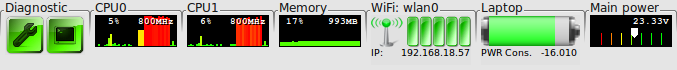
\includegraphics[width=13cm]{../../Common/img/ros/elektron_dashboard}
\caption[Okno interfejsu diagnostycznego]{Okno interfejsu diagnostycznego. W
kolejności od lewej: przywołanie okna wyświetlającego dokładne komunikaty z modułów diagnostycznych, przywołanie
konsoli z komunikatami systemu ROS, obciążenie procesora (dwa rdzenie), stan
pamięci RAM, poziom sygnału sieci bezprzewodowej, stan naładowania akumulatora
laptopa oraz napięcie na akumulatorach robota.}
\label{fig:elektron_dashboard}
\end{figure}
